\section{Using Catalyst}
\label{sec:catalyst}

Catalyst is the extensible and flexible coprocessing library of ParaView. 
It has been designed to be tightly coupled with simulation codes to perform in situ analysis at run time. 
Catalyst leverages the Visualization Toolkit (VTK) for scalable data analysis and visualization. Furthermore, it can be coupled with the ParaView In Situ Analysis framework to perform run-time visualization of data extracts and steering of the data analysis pipeline.

Catalyst provides two sets of tools: one for simulation users and one for simulation developers.
For simulation users, it is possible to create a coprocessing pipeline using two different methods. 
The first method does not require any knowledge of ParaView and relies on pre-generated scripts. These predefined scripts can be written in C++ or Python and are, usually, expected to run without any configuration options. 
The second method uses the ParaView interface to generate a coprocessing script from scratch and intuitively adjust its parameters as needed. This method is similar to using ParaView interactively to setup desired post-processing pipelines. The goal of these pipelines is to extract post-processed information during the simulation run. Ideally one should start with a representative dataset from the simulation. It is also possible to modify directly the generated Python's scripts which have been previously created using ParaView. However, this would require a knowledge of the ParaView Python API.

For simulation developers, Catalyst provides the tools to create an adaptor between the simulation code and the visualization pipeline.
The adaptor binds the simulation code and Catalyst so that both the functions of the simulation code and the general-purpose application programming interface (API) of Catalyst can be accessed. As Catalyst itself is independent of the simulation code, only the adaptor has to be developed by the designers of the solver. This flexibility is critical in order to successfully integrate external code into complex simulations usually running with different languages and packages. Catalyst is also easily extensible so that users can deploy new analysis and visualization techniques to existing coprocessing installations. Catalyst provides all the communication and synchronization routine and the pipeline mechanics necessary for coprocessing. Catalyst also provides powerful data processing capabilities through VTK filters as well as many writers and support for compositing and rendering.

Catalyst has also been developed with features to address limitations that come with pre-configuring a pipeline, but there may still be some unexpected data in the arbitrary simulation. To address these situations, the pipeline must be adjusted interactively.
The Catalyst library can leverage ParaView's client server mechanism to allow an interactive ParaView client to connect to a server running inside an in situ pipeline. ParaView can then read from a Catalyst data source like it reads from a file. This offers to construct/modify a pipeline interactively in the ParaView client via this live data source. Additionally, by enabling the client-server architecture in the Catalyst library, some or all of the data analysis and visualization pipeline can offload, if desired, to a separate machine, e.g., a smaller visualization cluster with specialized graphics hardware.

~\
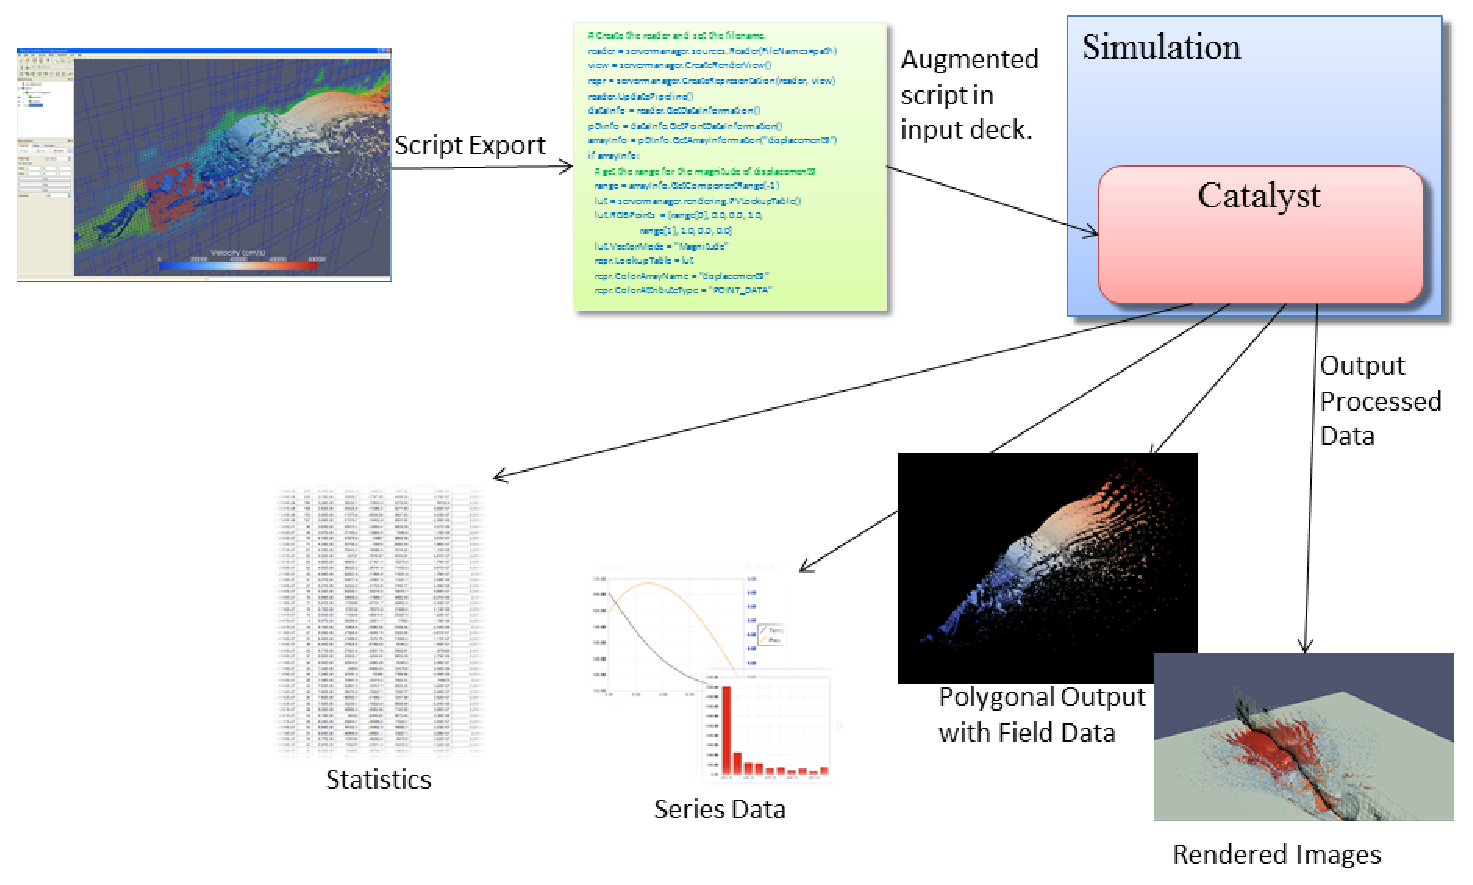
\includegraphics[scale=0.65]{pictures/CatalystFullWorkFlow.eps}
\captionof{figure}{Overall Catalyst workflow.}
\label{fig:catalyst}
\vspace{+0.04in}
~\

\subsection{Code\_Saturne with Catalyst}

\subsubsection{Adaptor implementation}
Typically, computational resource requirements are primarily determined either by the time to solution,
or the size of the model. For time to solution, the number of cores is selected in order to solve the problem in a given time. For size of model, the number of cores is selected in order to the model into available memory. 
When embedding Catalyst there is always a non-zero cost in terms of time, memory and the number of processors. Naively, one could simply
address these issues by simply requesting a greater number of processors, but in most cases this simply is
not possible or practical. Therefore, great care must be taken in the construction of the adaptors.
If memory is limited, the adaptor either uses complicated pointer manipulation or uses a smaller region
of memory. If memory is not limited, then deep copy of the simulation data structures into a VTK
data object doubles the resident memory, but also creates a CPU cost involved with copying data.
The overriding overhead issue in embedding ParaView Catalyst in a simulation code is the memory
management in an adaptor translating data structures in the running simulation.

In order to coprocess the simulation data, Catalyst must be provided with the
data formatted to the VTK data object structure. To accomplish this, several
solutions are possible, essentially depending on the format used for the data
of the simulation code. In the case when the format of the simulation code is
similar to VTK  and, moreover, the simulation data can be shared at any time,
then it is possible to feed Catalyst with a direct pointer to the simulation
memory. This option is indeed preferred, when possible, as it allows to decrease the memory footprint.
Another option is to fully or partially copy the data from the
simulation into a VTK object, and then send this object to Catalyst.

As users of Code\_Saturne are provided with several output formats and as the data
structure in our simulation differs from the VTK data object structure, feeding
Catalyst with a direct pointer to the simulation memory is not possible. Thus, in this configuration
data is copied from the simulation into a VTK data object. In fact, we
 allocate a vtkDoubleArray data structure to store our data for Catalyst. Furthermore, we
provide a pointer of this VTK data structure to Code\_Saturne so it can transform
its simulation data and then fill the VTK data object.

The memory cost increase of our solution can be alleviated by using more
machines. The CPU cost of the copy is in a range similar to the one needed when
adapting simulation data to a specific output format. This cost is largely
affordable comparatively to the time to write data to disk when storing time
step specific outputs. 

\subsubsection{Pipeline configuration}

From the point of view of an engineer performing a fluid mechanics simulation
using Code\_Saturne, the workflow of a coprocessing-simulation is 1) to define
a ParaView pipeline describing what the user wants to study and 2) to run the
simulation. Since users are already familiar with fluid mechanics
simulations, defining the pipeline for the coprocessing remains the main
sticking point. Thus this new process should be done in an efficient way and 
should not become a cumbersome bottleneck. This point is of great importance, especially in
an industrial environment like ours.

As we have explained in the previous section, the definition of a Catalyst pipeline can be achieve either 
programmatically or via the ParaView interface. In our industrial context, the former 
was considered too complicated and time consuming for the end user, especially when setting camera
parameters is needed, as no visualization feedback is provided. Therefore, the Catalyst pipeline has 
been created using the ParaView user's interface. This solution appears to be much easier as one
can simply interact with ParaView in the same way he/she uses to when
visualizing the results a posteriori. This solution is also easier to deploy with ParaView using the 
its companion coprocessing plugin. 

Indeed, using ParaView to define the coprocessing requires a representative input dataset.
One could use the available resources on a large cluster in order to setup the pipeline. However we chose to  
provide a simplified or under-sampled version of the large geometry to define the
pipeline. In fact, this strategy is possible in ParaView but some
characteristics of the initial geometry must be present in its simplified version; more importantly the name of the data fields must
remain the same, as they are part of the definition of the pipeline.

The generation of the coprocessing pipeline implies several steps.
First of all, the users start with a CAD (Computer Aided Design)
version of the geometry which is parametrized. This parametric representation
can generate meshes at different resolution levels. In our case, this is
performed inside the open-source SALOME~\cite{4291178} platform for numerical simulation. 

We then generate two different meshes, one at high resolution (up to 204M
hexahedrals in the current use cases) that will be used for the CFD
simulation and one with a lower resolution to define the pipeline (700 000
hexahedrals in our use cases). The lowest resolution mesh is fed into Code\_Saturne to perform a short
simulation. This allows ParaView to obtain a representation containing not
only the geometry but also the result fields. This is the data that is then used to define the pipeline.
The different processing pipelines are presented next.
